\chapter{Analisi dei requisiti}
\label{cap:analisi-requisiti}

\intro{In questa sezione vengono analizzati i requisiti del progetto e ne viene data un’analisi ad alto livello, combinando
una visione concettuale con una visione pratica ed implementativa. Vengono inoltre descritti i casi d’uso e i requisiti
individuati, con l’obiettivo di fornire una visione generale del sistema e delle sue funzionalità, in modo semplice e
comprensibile.}\\

\section{Obiettivi dello stage}

Gli obiettivi fondamentali da raggiungere durante il periodo di tirocinio, stilati
in accordo con il tutor aziendale ed inseriti nel documento Piano di Lavoro, sono
identificati dalla seguente notazione:
\begin{itemize}
    \item \textbf{OO}: obiettivi obbligatori, vincolanti in quanto obiettivo primario richiesto dal committente;
    \item \textbf{OD}: obiettivi desiderabili, non vincolanti o strettamente necessari, ma dal riconoscibile valore aggiunto.
    \item \textbf{OZ}: obiettivi opzionali, non vincolanti e non necessari, ma che potrebbero essere implementati in un secondo momento.
\end{itemize}

Alle sigle precedentemente indicate seguirà un numero progressivo, identificando così
tutti gli obiettivi.\\
Essi sono i seguenti:
\begin{itemize}
    \item Obbligatori:
    \begin{itemize}
        \item \textbf{OO1}: acquisizione di competenze pratiche su Oribea/DialogSphere;
        \item \textbf{OO2}: connessione a database e gestione dati aziendali o pubblici;
        \item \textbf{OO3}: implementazione di un Task AI che genera un sistema di raccomandazioni e report automatico basato su analisi delle vendite;
        \item \textbf{OO4}: implementazione di un Task AI che permette di raccomandare prodotti ad un cliente in base ai suoi dati di vendita, e viceversa di raccomandare clienti ad un prodotto;
        \item \textbf{OO5}: generazione automatica di report con output coerente, chiaro e adattabile;
        \item \textbf{OO6}: testing e documentazione completa del prototipo.
    \end{itemize}
    \item Desiderabili:
    \begin{itemize}
        \item \textbf{OD1}: ottimizzazione del Task AI per performance e scalabilità;
        \item \textbf{OD2}: personalizzazione dinamica dei prompt per casi d’uso differenti;
        \item \textbf{OD3}: integrazione con strumenti di visualizzazione o interfacce utente.
    \end{itemize}
    \item Opzionali:
    \begin{itemize}
        \item \textbf{OZ1}: sviluppo di un chatbot o di una dashboard interattiva per l'interazione con il sistema di raccomandazioni e report;
        \item \textbf{OZ2}: sperimentazione di tecniche di Explainable AI (XAI) per la trasparenza dei risultati;
        \item \textbf{OZ3}: esportazione automatica dei report in PDF/HTML o invio via e-mail.
    \end{itemize}
\end{itemize}


\section{Casi d'uso}

Per lo studio dei casi di utilizzo delle due task sono stati creati dei diagrammi.\\
I diagrammi dei casi d'uso (in inglese \emph{Use Case Diagram}) sono diagrammi di tipo \gls{uml} dedicati alla descrizione delle funzioni o servizi offerti da un sistema, così come sono percepiti e utilizzati dagli attori che interagiscono col sistema stesso. Nel mio caso, l'unico attore che interagisce con le due task è l'utente semplice, che rappresenta un generico utente autenticato nella piattaforma Oribea.\\
Ciascun caso d’uso riporta gli attori coinvolti, le sue precondizioni, la sua descrizione, le sue postcondizioni ed eventuali sottocasi d’uso, inclusioni, specializzazioni e
scenari alternativi.\\
I casi d’uso che sono stati definiti sono i seguenti:


\begin{usecase}{1}{Caricamento file CSV}

\begin{figure}[!h] 
    \centering 
    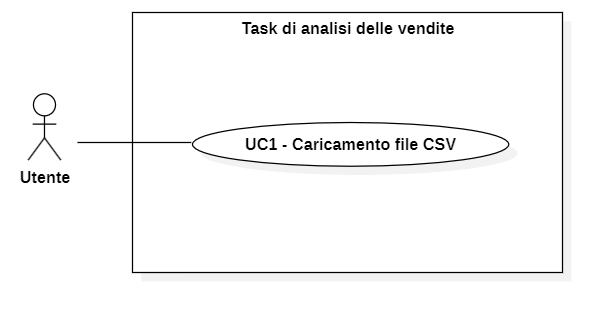
\includegraphics[width=0.9\columnwidth]{usecase/UC1 - Caricamento file CSV.png}
    \caption{UC1 - Caricamento file CSV}
\end{figure}

\usecaseactors{Utente}
\usecasepre{L'utente ha avviato la task di analisi delle vendite}
\usecasedesc{L'utente carica un file CSV contenente i dati delle vendite}
\usecasepost{Il sistema ha caricato il file CSV e lo ha memorizzato in un database Google Cloud}
\label{uc:caricamento-file-csv}
\end{usecase}


\begin{usecase}{2}{Selezione lingua per il report}

\begin{figure}[!h] 
    \centering 
    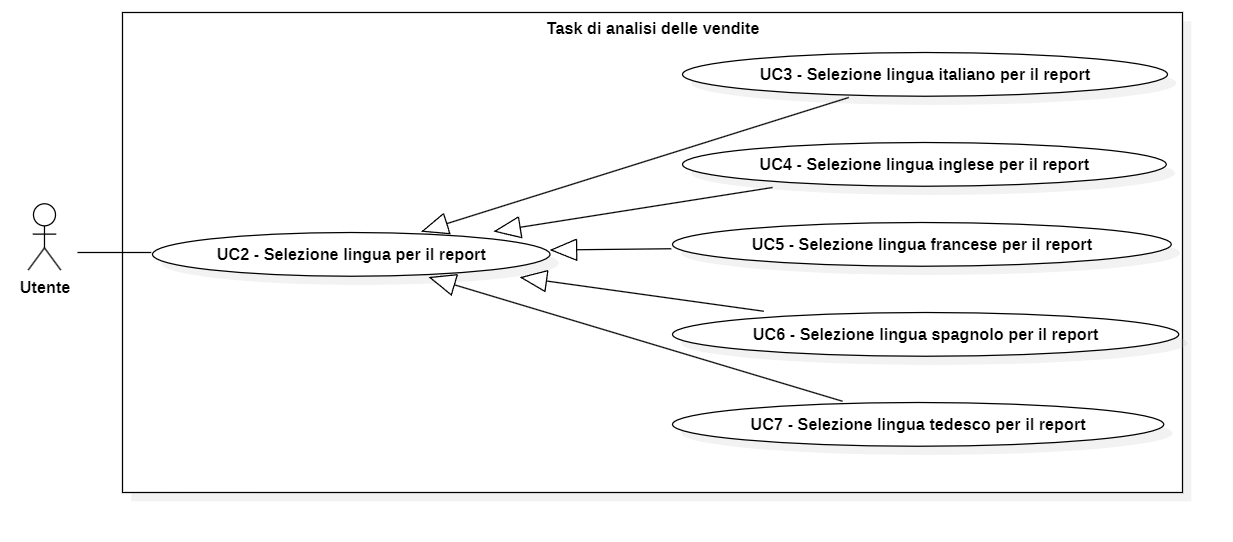
\includegraphics[width=0.9\columnwidth]{usecase/UC2 - Selezione lingua per il report.png}
    \caption{UC2 - Selezione lingua per il report}
\end{figure}

\usecaseactors{Utente}
\usecasepre{L'utente ha avviato la task di analisi delle vendite}
\usecasedesc{L'utente seleziona la lingua in cui desidera generare il report}
\usecasepost{Il sistema ha memorizzato la lingua selezionata}
\usespecial{UC3, UC4, UC5, UC6, UC7}
\label{uc:selezione-lingua-report}
\end{usecase}


\begin{usecase}{3}{Selezione lingua italiano per il report}

\usecaseactors{Utente}
\usecasepre{L'utente ha avviato la task di analisi delle vendite}
\usecasedesc{L'utente seleziona la lingua italiano perchè desidera generare il report in italiano}
\usecasepost{Il sistema ha memorizzato la lingua italiano selezionata}
\label{uc:selezione-lingua-italiano-report}
\end{usecase}


\begin{usecase}{4}{Selezione lingua inglese per il report}

\usecaseactors{Utente}
\usecasepre{L'utente ha avviato la task di analisi delle vendite}
\usecasedesc{L'utente seleziona la lingua inglese perchè desidera generare il report in inglese}
\usecasepost{Il sistema ha memorizzato la lingua inglese selezionata}
\label{uc:selezione-lingua-inglese-report}
\end{usecase}


\begin{usecase}{5}{Selezione lingua francese per il report}

\usecaseactors{Utente}
\usecasepre{L'utente ha avviato la task di analisi delle vendite}
\usecasedesc{L'utente seleziona la lingua francese perchè desidera generare il report in francese}
\usecasepost{Il sistema ha memorizzato la lingua francese selezionata}
\label{uc:selezione-lingua-francese-report}
\end{usecase}


\begin{usecase}{6}{Selezione lingua spagnolo per il report}

\usecaseactors{Utente}
\usecasepre{L'utente ha avviato la task di analisi delle vendite}
\usecasedesc{L'utente seleziona la lingua spagnolo perchè desidera generare il report in spagnolo}
\usecasepost{Il sistema ha memorizzato la lingua spagnolo selezionata}
\label{uc:selezione-lingua-spagnolo-report}
\end{usecase}


\begin{usecase}{7}{Selezione lingua tedesco per il report}

\usecaseactors{Utente}
\usecasepre{L'utente ha avviato la task di analisi delle vendite}
\usecasedesc{L'utente seleziona la lingua tedesco perchè desidera generare il report in tedesco}
\usecasepost{Il sistema ha memorizzato la lingua tedesco selezionata}
\label{uc:selezione-lingua-tedesco-report}
\end{usecase}


\begin{usecase}{8}{Selezione valuta per il report}

\begin{figure}[!h] 
    \centering 
    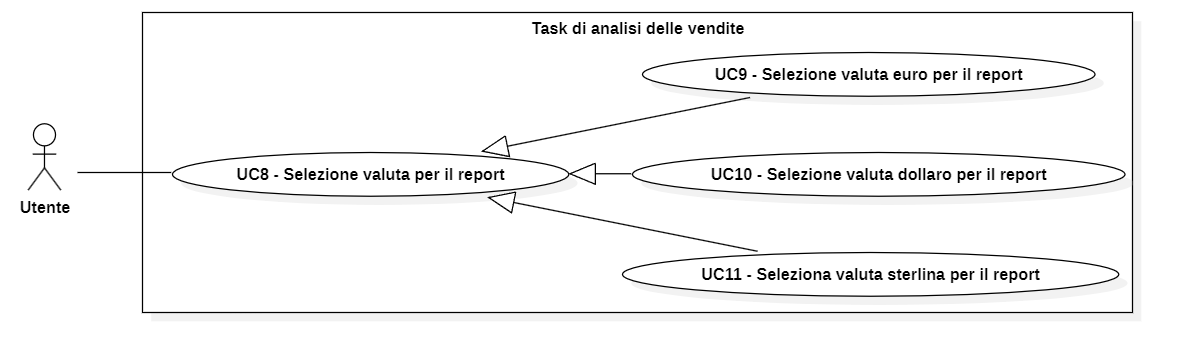
\includegraphics[width=0.9\columnwidth]{usecase/UC8 - Selezione valuta per il report.png}
    \caption{UC8 - Selezione valuta per il report}
\end{figure}

\usecaseactors{Utente}
\usecasepre{L'utente ha avviato la task di analisi delle vendite}
\usecasedesc{L'utente seleziona la valuta in cui desidera generare il report}
\usecasepost{Il sistema ha memorizzato la valuta selezionata}
\usespecial{UC9, UC10, UC11}
\label{uc:selezione-valuta-report}
\end{usecase}


\begin{usecase}{9}{Selezione valuta euro per il report}

\usecaseactors{Utente}
\usecasepre{L'utente ha avviato la task di analisi delle vendite}
\usecasedesc{L'utente seleziona la valuta euro perchè desidera generare il report con i valori monetari espressi in euro}
\usecasepost{Il sistema ha memorizzato la valuta euro selezionata}
\label{uc:selezione-valuta-euro-report}
\end{usecase}


\begin{usecase}{10}{Selezione valuta dollaro per il report}

\usecaseactors{Utente}
\usecasepre{L'utente ha avviato la task di analisi delle vendite}
\usecasedesc{L'utente seleziona la valuta dollaro perchè desidera generare il report con i valori monetari espressi in dollari}
\usecasepost{Il sistema ha memorizzato la valuta dollaro selezionata}
\label{uc:selezione-valuta-dollaro-report}
\end{usecase}


\begin{usecase}{11}{Selezione valuta sterlina per il report}

\usecaseactors{Utente}
\usecasepre{L'utente ha avviato la task di analisi delle vendite}
\usecasedesc{L'utente seleziona la valuta sterlina perchè desidera generare il report con i valori monetari espressi in sterline}
\usecasepost{Il sistema ha memorizzato la valuta sterlina selezionata}
\label{uc:selezione-valuta-sterlina-report}
\end{usecase}


\begin{usecase}{12}{Visualizzazione risultato della task}

\begin{figure}[!h]
    \centering 
    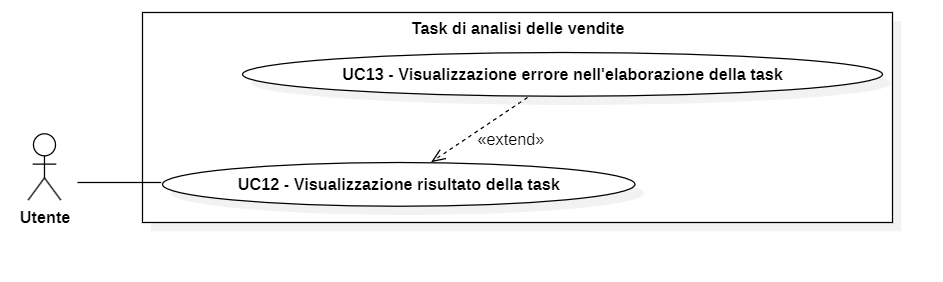
\includegraphics[width=0.9\columnwidth]{usecase/UC12 - Visualizzazione risultato della task.png}
    \caption{UC12 - Visualizzazione risultato della task}
\end{figure}

\usecaseactors{Utente}
\usecasepre{L'utente ha cliccato sul pulsante di esecuzione della task di analisi delle vendite}
\usecasedesc{L'utente visualizza il risultato della task di analisi delle vendite}
\usecasepost{L'utente ha visualizzato il risultato della task di analisi delle vendite}
\usecasealt{UC13}
\useinclu{UC12.1, UC12.2, UC12.3, UC12.4}  % Ricordati di modificare qua, se dovesse cambiare qualcosa
\label{uc:visualizzazione-risultato-task}
\end{usecase}


% 12.1, 12.2, 12.3 e 12.4 non li metto ancora perchè ho una domanda


\begin{usecase}{13}{Visualizzazione errore nell'elaborazione della task}

\usecaseactors{Utente}
\usecasepre{L'utente ha cliccato sul pulsante di esecuzione della task di analisi delle vendite}
\usecasedesc{L'utente visualizza un errore nell'elaborazione della task di analisi delle vendite}
\usecasepost{L'utente ha visualizzato un errore nell'elaborazione della task di analisi delle vendite}
\label{uc:visualizzazione-errore-task}
\end{usecase}


% UC14, UC15, e UC16 non li metto ancora perchè ho una domanda


\begin{usecase}{17}{Inserimento del nome del file CSV degli ordini originale}

\begin{figure}[!h] 
    \centering 
    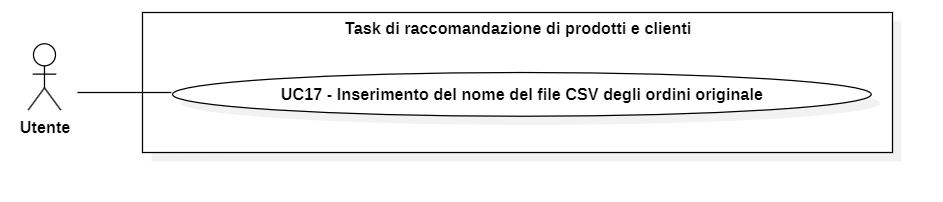
\includegraphics[width=0.9\columnwidth]{usecase/UC17 - Inserimento nome CSV degli ordini originale.png}
    \caption{UC17 - Inserimento del nome del file CSV degli ordini originale}
\end{figure}

\usecaseactors{Utente}
\usecasepre{L'utente ha avviato la task di raccomandazione di prodotti e clienti}
\usecasedesc{L'utente inserisce il nome del file CSV degli ordini originale}
\usecasepost{Il sistema ricerca il file CSV corrispondente al nome inserito all'interno del database Google Cloud}
\label{uc:inserimento-nome-file-csv}
\end{usecase}


\begin{usecase}{18}{Selezione tipo di raccomandazione}

\begin{figure}[!h] 
    \centering 
    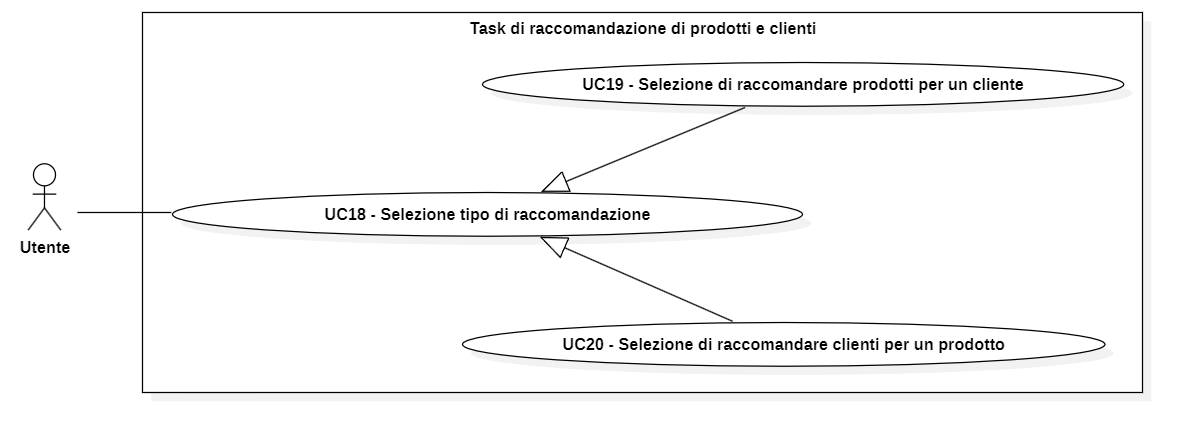
\includegraphics[width=0.9\columnwidth]{usecase/UC18 - Selezione tipo di raccomandazione.png}
    \caption{UC18 - Selezione tipo di raccomandazione}
\end{figure}

\usecaseactors{Utente}
\usecasepre{L'utente ha avviato la task di raccomandazione di prodotti e clienti}
\usecasedesc{L'utente seleziona la tipologia di raccomandazione che desidera che venga eseguita}
\usecasepost{Il sistema ha memorizzato il tipo di raccomandazione selezionato}
\usespecial{UC19, UC20}
\label{uc:selezione-tipo-elemento}
\end{usecase}


\begin{usecase}{19}{Selezione di raccomandare prodotti per un cliente}

\usecaseactors{Utente}
\usecasepre{L'utente ha avviato la task di raccomandazione di prodotti e clienti}
\usecasedesc{L'utente seleziona il tipo di raccomandazione "raccomandare prodotti per un cliente"}
\usecasepost{Il sistema ha memorizzato il tipo di raccomandazione "raccomandare prodotti per un cliente" selezionato}
\label{uc:selezione-raccomandare-prodotti}
\end{usecase}


\begin{usecase}{20}{Selezione di raccomandare clienti per un prodotto}

\usecaseactors{Utente}
\usecasepre{L'utente ha avviato la task di raccomandazione di prodotti e clienti}
\usecasedesc{L'utente seleziona il tipo di raccomandazione "raccomandare clienti per un prodotto"}
\usecasepost{Il sistema ha memorizzato il tipo di raccomandazione "raccomandare clienti per un prodotto" selezionato}
\label{uc:selezione-raccomandare-clienti}
\end{usecase}


\begin{usecase}{21}{Inserimento nome elemento per cui raccomandare}

\begin{figure}[!h] 
    \centering 
    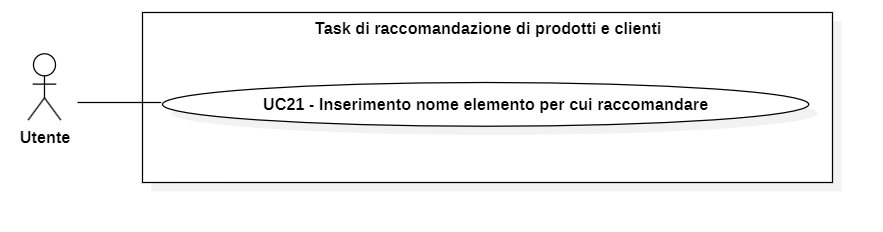
\includegraphics[width=0.9\columnwidth]{usecase/UC21 - Inserimento nome elemento a cui raccomandare.png}
    \caption{UC21 - Inserimento nome elemento per cui raccomandare}
\end{figure}

\usecaseactors{Utente}
\usecasepre{L'utente ha avviato la task di raccomandazione di prodotti e clienti}
\usecasedesc{L'utente inserisce il nome dell'elemento per cui desidera che venga eseguita la raccomandazione}
\usecasepost{Il sistema cerca l'elemento corrispondente al nome inserito all'interno del database Google Cloud}
\label{uc:inserimento-nome-elemento}
\end{usecase}


\begin{usecase}{22}{Selezione lingua per la raccomandazione}

\begin{figure}[!h] 
    \centering 
    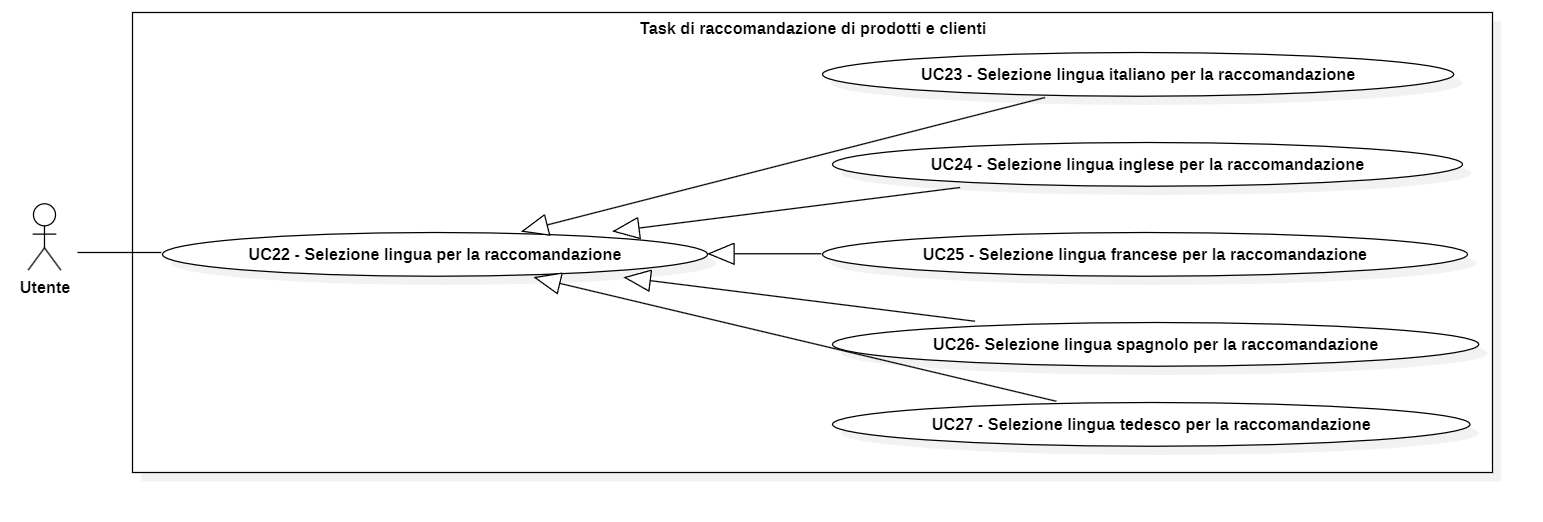
\includegraphics[width=0.9\columnwidth]{usecase/UC22 - Selezione lingua per la raccomandazione.png}
    \caption{UC22 - Selezione lingua per la raccomandazione}
\end{figure}

\usecaseactors{Utente}
\usecasepre{L'utente ha avviato la task di raccomandazione di prodotti e clienti}
\usecasedesc{L'utente seleziona la lingua in cui desidera generare la raccomandazione}
\usecasepost{Il sistema ha memorizzato la lingua selezionata}
\usespecial{UC23, UC24, UC25, UC26, UC27}
\label{uc:selezione-lingua-raccomandazione}
\end{usecase}


\begin{usecase}{23}{Selezione lingua italiano per la raccomandazione}

\usecaseactors{Utente}
\usecasepre{L'utente ha avviato la task di raccomandazione di prodotti e clienti}
\usecasedesc{L'utente seleziona la lingua italiano perchè desidera generare la raccomandazione in italiano}
\usecasepost{Il sistema ha memorizzato la lingua italiano selezionata}
\label{uc:selezione-lingua-italiano-raccomandazione}
\end{usecase}


\begin{usecase}{24}{Selezione lingua inglese per la raccomandazione}

\usecaseactors{Utente}
\usecasepre{L'utente ha avviato la task di raccomandazione di prodotti e clienti}
\usecasedesc{L'utente seleziona la lingua inglese perchè desidera generare la raccomandazione in inglese}
\usecasepost{Il sistema ha memorizzato la lingua inglese selezionata}
\label{uc:selezione-lingua-inglese-raccomandazione}
\end{usecase}


\begin{usecase}{25}{Selezione lingua francese per la raccomandazione}

\usecaseactors{Utente}
\usecasepre{L'utente ha avviato la task di raccomandazione di prodotti e clienti}
\usecasedesc{L'utente seleziona la lingua francese perchè desidera generare la raccomandazione in francese}
\usecasepost{Il sistema ha memorizzato la lingua francese selezionata}
\label{uc:selezione-lingua-francese-raccomandazione}
\end{usecase}


\begin{usecase}{26}{Selezione lingua spagnolo per la raccomandazione}

\usecaseactors{Utente}
\usecasepre{L'utente ha avviato la task di raccomandazione di prodotti e clienti}
\usecasedesc{L'utente seleziona la lingua spagnolo perchè desidera generare la raccomandazione in spagnolo}
\usecasepost{Il sistema ha memorizzato la lingua spagnolo selezionata}
\label{uc:selezione-lingua-spagnolo-raccomandazione}
\end{usecase}


\begin{usecase}{27}{Selezione lingua tedesco per la raccomandazione}

\usecaseactors{Utente}
\usecasepre{L'utente ha avviato la task di raccomandazione di prodotti e clienti}
\usecasedesc{L'utente seleziona la lingua tedesco perchè desidera generare la raccomandazione in tedesco}
\usecasepost{Il sistema ha memorizzato la lingua tedesco selezionata}
\label{uc:selezione-lingua-tedesco-raccomandazione}
\end{usecase}


\begin{usecase}{28}{Visualizzazione classifica elementi raccomandati}

\begin{figure}[!h] 
    \centering 
    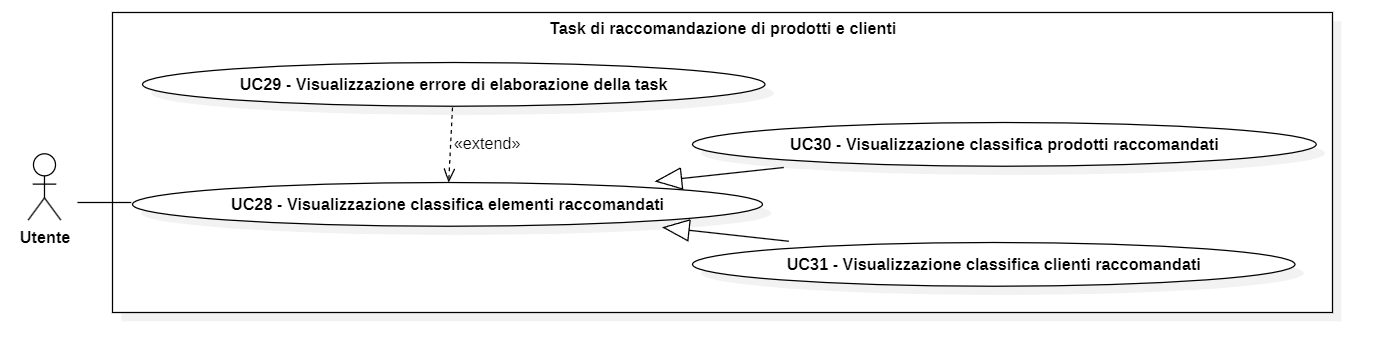
\includegraphics[width=0.9\columnwidth]{usecase/UC28 - Visualizzazione classifica elementi raccomandati.png}
    \caption{UC28 - Visualizzazione classifica elementi raccomandati}
\end{figure}

\usecaseactors{Utente}
\usecasepre{L'utente ha cliccato sul pulsante di esecuzione della task di raccomandazione di prodotti e clienti}
\usecasedesc{L'utente visualizza la classifica degli elementi raccomandati}
\usecasepost{L'utente ha visualizzato la classifica degli elementi raccomandati}
\usecasealt{UC29}
\usespecial{UC30, UC31}
\label{uc:visualizzazione-classifica-elementi-raccomandati}
\end{usecase}


\begin{usecase}{29}{Visualizzazione errore di elaborazione della task}

\usecaseactors{Utente}
\usecasepre{L'utente ha cliccato sul pulsante di esecuzione della task di raccomandazione di prodotti e clienti}
\usecasedesc{L'utente visualizza un errore nell'elaborazione della task di raccomandazione di prodotti e clienti}
\usecasepost{L'utente ha visualizzato un errore nell'elaborazione della task di raccomandazione di prodotti e clienti}
\label{uc:visualizzazione-errore-elaborazione-task}
\end{usecase}


\begin{usecase}{30}{Visualizzazione classifica prodotti raccomandati}

\usecaseactors{Utente}
\usecasepre{L'utente ha cliccato sul pulsante di esecuzione della task di raccomandazione di prodotti e clienti}
\usecasedesc{L'utente visualizza la classifica dei prodotti raccomandati}
\usecasepost{L'utente ha visualizzato la classifica dei prodotti raccomandati}
\label{uc:visualizzazione-classifica-prodotti-raccomandati}
\end{usecase}


\begin{usecase}{31}{Visualizzazione classifica clienti raccomandati}

\usecaseactors{Utente}
\usecasepre{L'utente ha cliccato sul pulsante di esecuzione della task di raccomandazione di prodotti e clienti}
\usecasedesc{L'utente visualizza la classifica dei clienti raccomandati}
\usecasepost{L'utente ha visualizzato la classifica dei clienti raccomandati}
\label{uc:visualizzazione-classifica-clienti-raccomandati}
\end{usecase}













\section{Tracciamento dei requisiti}

Da un'attenta analisi dei requisiti e degli use case effettuata sul progetto è stata stilata la tabella che traccia i requisiti in rapporto agli use case.\\
Sono stati individuati diversi tipi di requisiti e si è quindi fatto utilizzo di un codice identificativo per distinguerli.\\
Il codice dei requisiti è così strutturato R(F/Q/V)(N/D/O) dove:
\begin{enumerate}
	\item[R =] requisito
    \item[F =] funzionale
    \item[Q =] qualitativo
    \item[V =] di vincolo
    \item[N =] obbligatorio (necessario)
    \item[D =] desiderabile
    \item[Z =] opzionale
\end{enumerate}
Nelle tabelle \ref{tab:requisiti-funzionali}, \ref{tab:requisiti-qualitativi} e \ref{tab:requisiti-vincolo} sono riassunti i requisiti e il loro tracciamento con gli use case delineati in fase di analisi.

\newpage

\begin{table}%
\caption{Tabella del tracciamento dei requisti funzionali}
\label{tab:requisiti-funzionali}
\begin{tabularx}{\textwidth}{lXl}
\hline\hline
\textbf{Requisito} & \textbf{Descrizione} & \textbf{Use Case}\\
\hline
RFN-1     & L'interfaccia permette di configurare il tipo di sonde del test & UC1 \\
\hline
\end{tabularx}
\end{table}%

\begin{table}%
\caption{Tabella del tracciamento dei requisiti qualitativi}
\label{tab:requisiti-qualitativi}
\begin{tabularx}{\textwidth}{lXl}
\hline\hline
\textbf{Requisito} & \textbf{Descrizione} & \textbf{Use Case}\\
\hline
RQD-1    & Le prestazioni del simulatore hardware deve garantire la giusta esecuzione dei test e non la generazione di falsi negativi & - \\
\hline
\end{tabularx}
\end{table}%

\begin{table}%
\caption{Tabella del tracciamento dei requisiti di vincolo}
\label{tab:requisiti-vincolo}
\begin{tabularx}{\textwidth}{lXl}
\hline\hline
\textbf{Requisito} & \textbf{Descrizione} & \textbf{Use Case}\\
\hline
RVO-1    & La libreria per l'esecuzione dei test automatici deve essere riutilizzabile & - \\
\hline
\end{tabularx}
\end{table}%
